\subsection{CS-Status Module}
\par{Each user on the forum has a user status termed CS-Status. A users status (CS-Status) is determined by the role(s) he/she plays in one or more course modules. Thus from a persons CS-Status we are able to filter out what privileges the person should have on the forum and for which course modules.}
\subsubsection{Scope}
\par{The CS-Status of a user will be used for authorization purposes on the forum. Users of higher statuses will be able to perform additional actions on the forum that stock-users will not be able to perform.}
\subsubsection{Use cases}
\subsubsection*{Create CS Status}
\par{Upon login, the users CS-Status will be queried from LDAP and the local copy of the state of the user will be overwritten (for safety and efficiency). This ensures that any changes that may have taken place (updates to the users state) are persisted to our local databases.}
\subsubsection*{Get Status Symbol}
\par{When the user information is fetched from LDAP, the state of the user (for each of their course modules) must be transfered to an instance of the CS-Status module.}
\subsubsection{Domain model}
\par{The figure of the CS-Status domain model is in figure ~\ref{fig:cs}.}
\begin{figure}[h!]
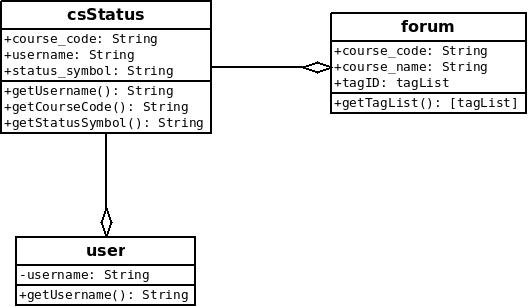
\includegraphics[width=\linewidth]{Diagrams/csStatus_domain_model.jpeg}
\caption{Domain model representing the CS status model}
\label{fig:cs}
\end{figure}
